\documentclass[12pt]{article}

% TEMPLATE DEFAULT PACKAGES
\usepackage{amssymb,amsmath,amsfonts,eurosym,geometry,ulem,graphicx,color,setspace,sectsty,comment,natbib,pdflscape,array,adjustbox}

% ADDED PACKAGES FOR THIS MANUSCRIPT
\usepackage{palatino,newtxmath,multirow,titlesec,threeparttable,tabu,booktabs,titlesec,threeparttable,mathtools,bm,bbm,subcaption,pdflscape,tcolorbox,mathrsfs}
% endfloat,

\usepackage{afterpage}
\usepackage[hyphens]{url}
\usepackage[margin=1cm]{caption}

\usepackage[draft]{hyperref}
\newcommand{\tim}{$\,\times\,$}
% FIGURES & TABLES CAPTION STYLING
\captionsetup[figure]{labelfont={bf},name={Figure},labelsep=period}
\captionsetup[table]{labelfont={bf},name={Table},labelsep=period}

% SECTION TITLE SETTINGS
\titlelabel{\thetitle.\enskip}
\titleformat*{\section}{\large\bfseries}
\titleformat*{\subsection}{\normalsize\bfseries}

% COLUMN TYPES
\newcolumntype{L}[1]{>{\raggedright\let\newline\\\arraybackslash\hspace{0pt}}m{#1}}
\newcolumntype{C}{>{\centering\arraybackslash}p{5.2em}}
\newcolumntype{D}{>{\centering\arraybackslash}p{5em}}
\newcolumntype{R}[1]{>{\raggedleft\let\newline\\\arraybackslash\hspace{0pt}}m{#1}}


% MARGINS AND SPACING
\normalem
\geometry{left=1.1in,right=1.1in,top=1.0in,bottom=1.0in}
\setlength{\parskip}{2.5pt}

% SPECIAL CELL 
\newcommand{\specialcell}[2][c]{%
	\begin{tabular}[#1]{@{}l@{}}#2\end{tabular}}

% NO INDENT ON FOOTNOTES
\usepackage[hang,flushmargin]{footmisc}

\begin{document}



% \vspace{0mm}
% \begin{table}[h!]
% \centering
% \caption{Housing Project Areas Description}\label{table:projectdescriptives}
% \vspace{0mm}
% \begin{tabular}{l*{1}{cccccc}}
% \toprule
%   & \multicolumn{2}{c}{\textbf{All}}& \multicolumn{2}{c}{\textbf{Greenfield}}  & \multicolumn{2}{c}{\textbf{In-Situ}}   \\
%   &Const. & Unconst. &Const. & Unconst.   & Const. & Unconst. \\
% \midrule
%  Number of Projects  & 172  & 145  & 43  & 20  & 27  & 29  \\ 
 Area (km2)  & 1.17  & 1.16  & 1.72  & 2.42  & 1.50  & 0.88  \\ 
 Median Construction Yr.  & 2006  & 2006  & 2006  & 2005  & 2004  & 2006  \\ 
 Delivered Houses  & 374  & 11  & 568  & 24  & 702  & 20  \\ 
 House Price in 1 km (R$^\dagger$)  & 188,441  & 218,635  & 194,214  & 186,841  & 179,596  & 208,570  \\ 
 Distance to CBD$^\ddagger$ (km)  & 32.5  & 27.7  & 40.5  & 39.9  & 32.6  & 30.6  \\ 

% \bottomrule
% \multicolumn{7}{l}{\scriptsize Const. refers to constructed projects and unconst. refers to unconstructed projects.}\\[-.5em]
% \multicolumn{7}{l}{\scriptsize $^*$Calculated from {\it expected} completion dates using Gauteng National Treasury budget reports.}\\[-.5em]
% \multicolumn{7}{l}{\scriptsize $^\dagger$ The USD averaged to about 7.70 Rands during the 2001-2011 period.}\\[-.5em]
% \multicolumn{7}{l}{\scriptsize $^\ddagger$Measured as the average minimum distance with respect to Johannesburg and Pretoria CBDs. } \\[-.5em]
% %\multicolumn{7}{l}{\scriptsize City includes projects whose centroids are within 30.4 km of their nearest CBD.} \\[-.5em]
% %\multicolumn{7}{l}{\scriptsize Suburb includes projects whose centroids are further than 30.4 km from their nearest CBD.}
% \end{tabular}
% \end{table} 



% \begin{figure*}
%         \centering
%    %     \caption[ Pre-Period Housing Densities in Constructed and Unconstructed Projects Areas ]
%   %      {\small Pre-Period Densities} 
%         %\vspace{2mm}
%         \begin{subfigure}[b]{0.48\textwidth}
%                     \caption[Network2]%
%             {{\footnotesize \textbf{All Projects} pre-period formal raw data}}    
%             \label{fig:prefor}
%             \centering
%             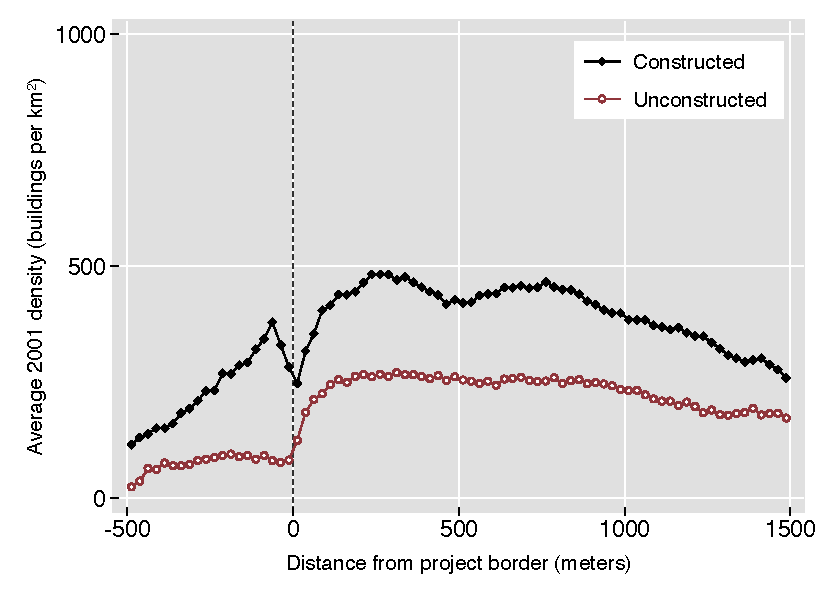
\includegraphics[width=\textwidth,trim={0.3cm .3cm 0.1cm 0cm}, clip=true]{figures/bblu_for_pre_means_4_spk.pdf}

%         \end{subfigure}
%         \hfill
%         \begin{subfigure}[b]{0.48\textwidth}  
%                     \caption[]%
%             {{\footnotesize \textbf{All Projects} pre-period informal  raw data}}      
%             \label{fig:preinf}
%             \centering 
%             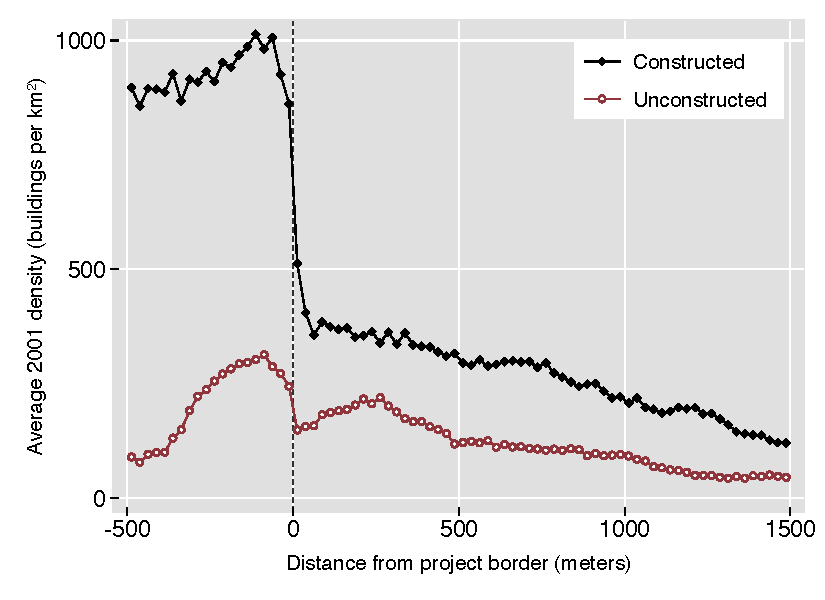
\includegraphics[width=\textwidth,trim={0.3cm .3cm 0.1cm 0cm}, clip=true]{figures/bblu_inf_pre_means_4_spk.pdf}

%         \end{subfigure}
%         \begin{subfigure}[b]{0.48\textwidth}
%                     \caption[Network2]%
%             {{\footnotesize \textbf{Greenfield} pre-period formal  raw data}}    
%             \label{fig:prefor}
%             \centering
%             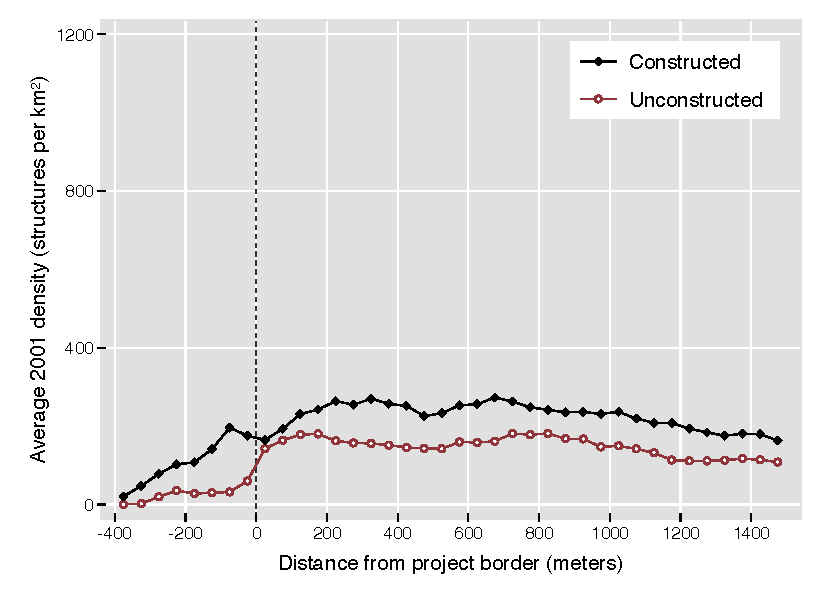
\includegraphics[width=\textwidth,trim={0.3cm .3cm 0.1cm 0cm}, clip=true]{figures/bblu_for_pre_means_4_1_spk.pdf}

%         \end{subfigure}
%         \hfill
%         \begin{subfigure}[b]{0.48\textwidth}  
%                     \caption[]%
%             {{\footnotesize \textbf{Greenfield} pre-period informal  raw data}}     
%             \label{fig:preinf}
%             \centering 
%             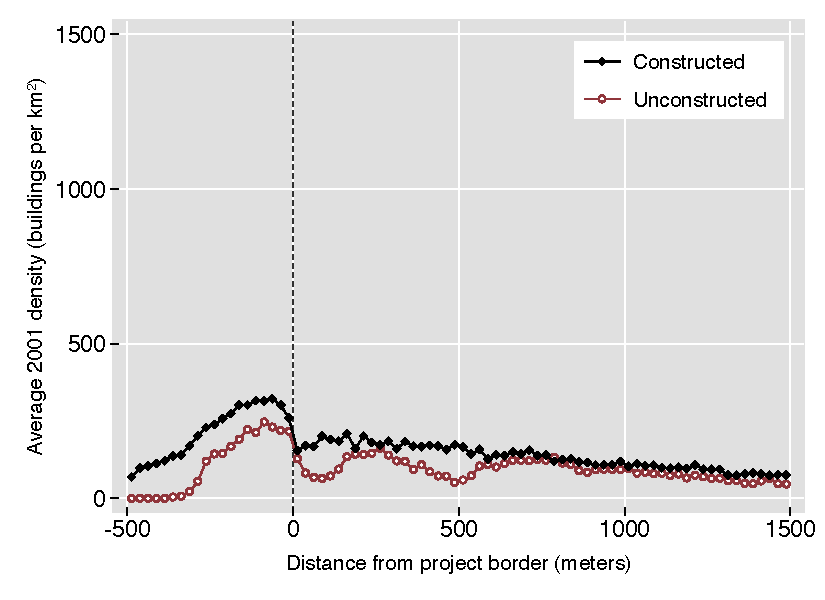
\includegraphics[width=\textwidth,trim={0.3cm .3cm 0.1cm 0cm}, clip=true]{figures/bblu_inf_pre_means_4_1_spk.pdf}

%         \end{subfigure}
%         \begin{subfigure}[b]{0.48\textwidth}
%                     \caption[Network2]%
%             {{\footnotesize \textbf{In-Situ} pre-period formal  raw data}}   
%             \label{fig:prefor}
%             \centering
%             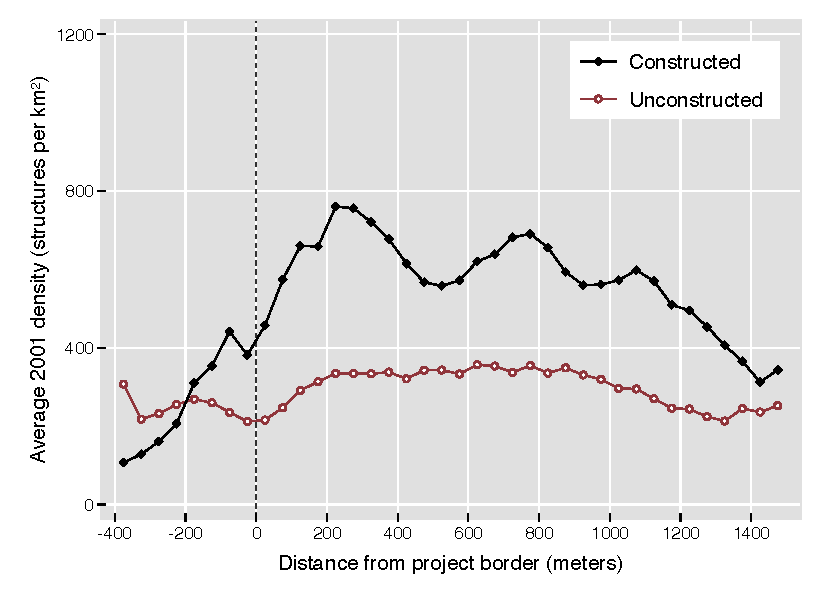
\includegraphics[width=\textwidth,trim={0.3cm .3cm 0.1cm 0cm}, clip=true]{figures/bblu_for_pre_means_4_2_spk.pdf}

%         \end{subfigure}
%         \hfill
%         \begin{subfigure}[b]{0.48\textwidth}  
%                     \caption[]%
%             {{\footnotesize \textbf{In-Situ} pre-period informal  raw data}}     
%             \label{fig:preinf}
%             \centering 
%             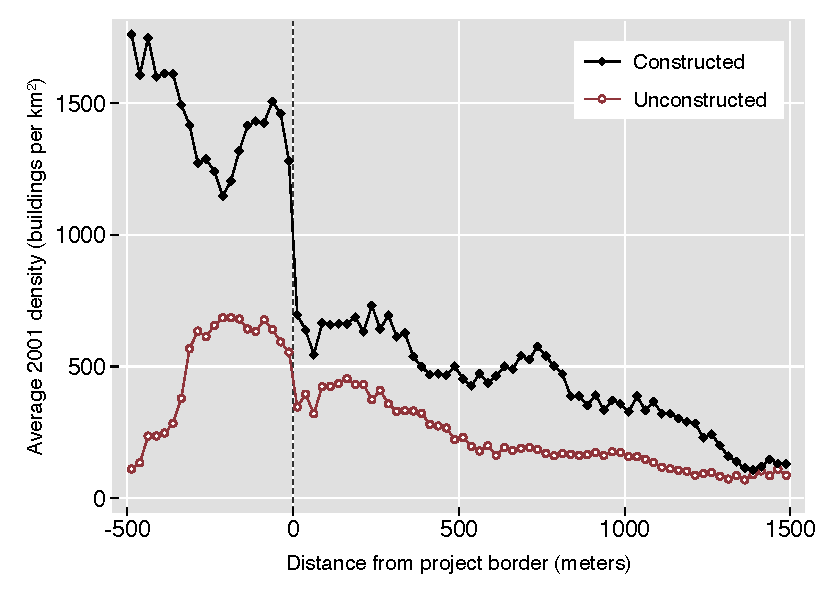
\includegraphics[width=\textwidth,trim={0.3cm .3cm 0.1cm 0cm}, clip=true]{figures/bblu_inf_pre_means_4_2_spk.pdf}

%         \end{subfigure}
%         \begin{subfigure}[b]{0.48\textwidth}
%                     \caption[Network2]%
%             {{\footnotesize \textbf{Other} pre-period formal  raw data}}   
%             \label{fig:prefor}
%             \centering
%             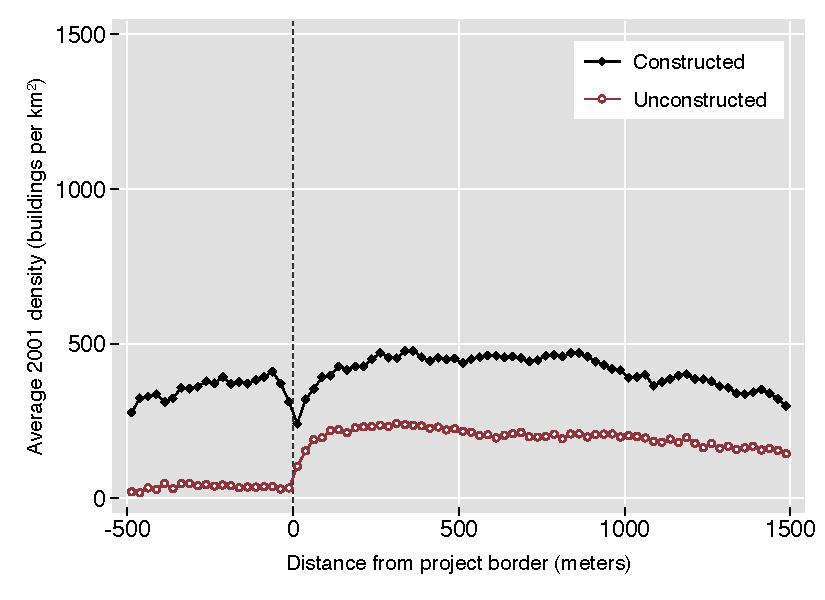
\includegraphics[width=\textwidth,trim={0.3cm .3cm 0.1cm 0cm}, clip=true]{figures/bblu_for_pre_means_4_3_spk.pdf}

%         \end{subfigure}
%         \hfill
%         \begin{subfigure}[b]{0.48\textwidth}  
%                     \caption[]%
%             {{\footnotesize \textbf{Other} pre-period informal  raw data}}      
%             \label{fig:preinf}
%             \centering 
%             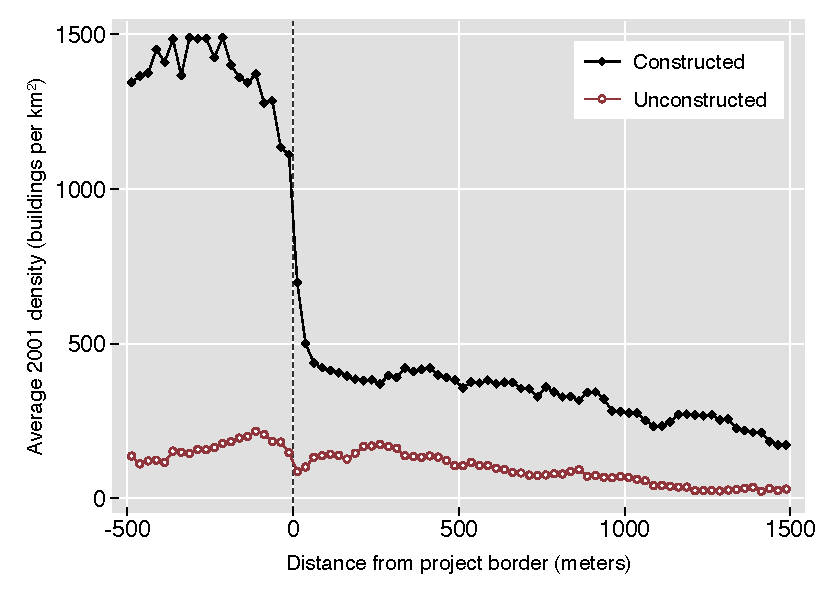
\includegraphics[width=\textwidth,trim={0.3cm .3cm 0.1cm 0cm}, clip=true]{figures/bblu_inf_pre_means_4_3_spk.pdf}

%         \end{subfigure}
% \end{figure*}








% \begin{figure*}
%         \centering
%    %     \caption[ Pre-Period Housing Densities in Constructed and Unconstructed Projects Areas ]
%   %      {\small Pre-Period Densities} 
%         %\vspace{2mm}
%         \begin{subfigure}[b]{0.48\textwidth}
%             \caption[Network2]%
%             {{\footnotesize \textbf{All Projects} changes formal raw data}}    
%             \label{fig:prefor}
%             \centering
%             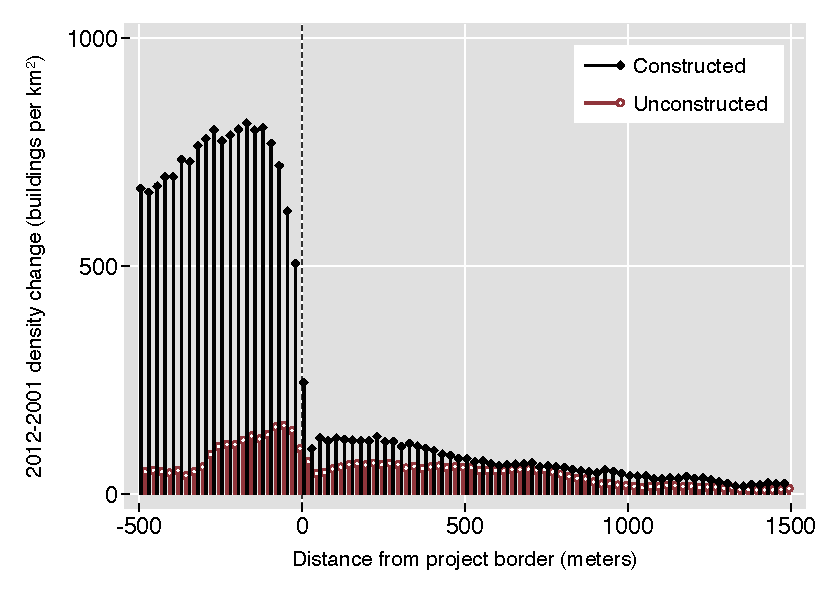
\includegraphics[width=\textwidth,trim={0.3cm .3cm 0.1cm 0cm}, clip=true]{figures/bblu_for_rawchanges_4_spk.pdf}

%         \end{subfigure}
%         \hfill
%         \begin{subfigure}[b]{0.48\textwidth}  
%                     \caption[]%
%             {{\footnotesize \textbf{All Projects} changes informal  raw data}}      
%             \label{fig:preinf}
%             \centering 
%             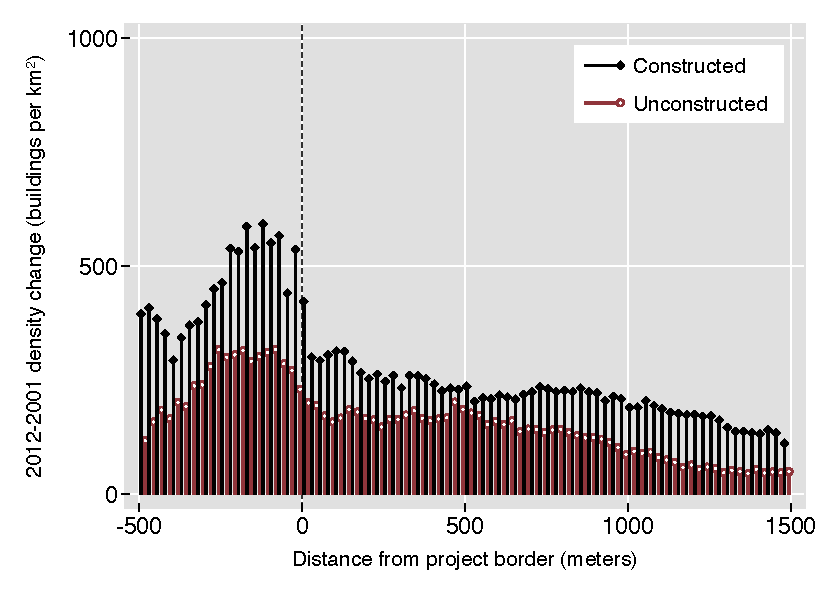
\includegraphics[width=\textwidth,trim={0.3cm .3cm 0.1cm 0cm}, clip=true]{figures/bblu_inf_rawchanges_4_spk.pdf}

%         \end{subfigure}
%         \begin{subfigure}[b]{0.48\textwidth}
%                     \caption[Network2]%
%             {{\footnotesize \textbf{Greenfield} changes formal  raw data}}    
%             \label{fig:prefor}
%             \centering
%             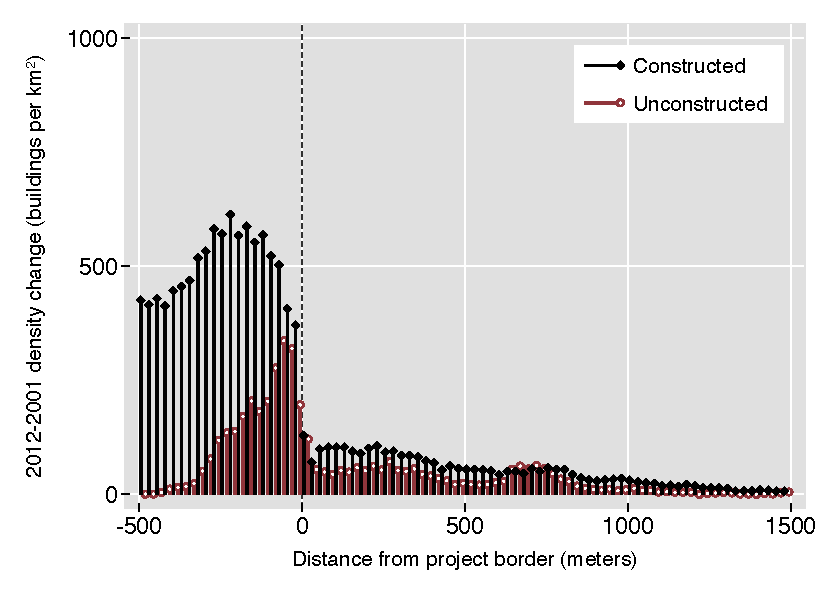
\includegraphics[width=\textwidth,trim={0.3cm .3cm 0.1cm 0cm}, clip=true]{figures/bblu_for_rawchanges_4_1_spk.pdf}

%         \end{subfigure}
%         \hfill
%         \begin{subfigure}[b]{0.48\textwidth}  
%                     \caption[]%
%             {{\footnotesize \textbf{Greenfield} changes informal raw data }}     
%             \label{fig:preinf}
%             \centering 
%             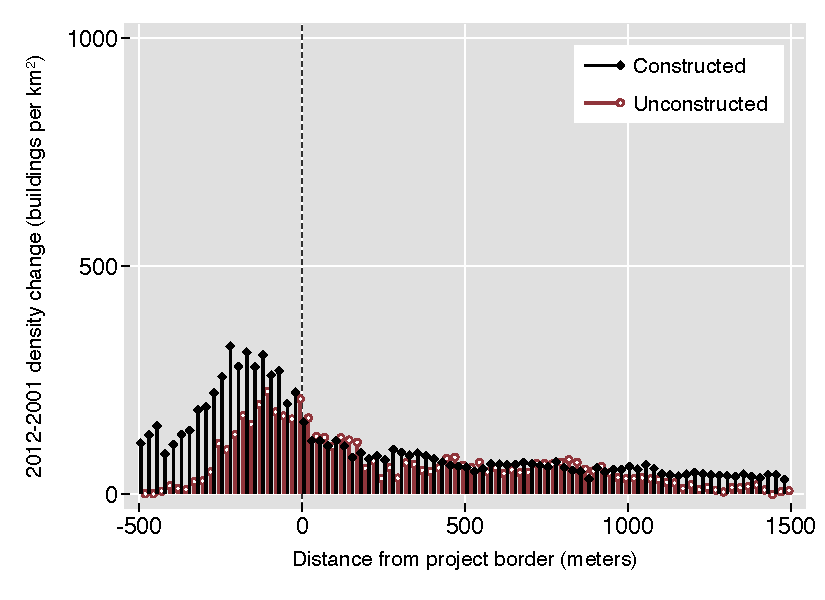
\includegraphics[width=\textwidth,trim={0.3cm .3cm 0.1cm 0cm}, clip=true]{figures/bblu_inf_rawchanges_4_1_spk.pdf}

%         \end{subfigure}
%         \begin{subfigure}[b]{0.48\textwidth}
%                     \caption[Network2]%
%             {{\footnotesize \textbf{In-Situ} changes formal raw data }}   
%             \label{fig:prefor}
%             \centering
%             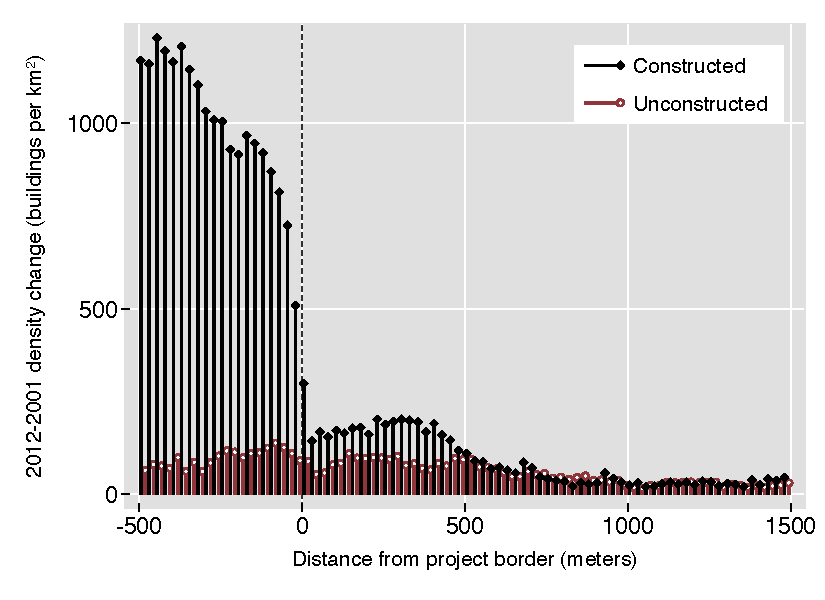
\includegraphics[width=\textwidth,trim={0.3cm .3cm 0.1cm 0cm}, clip=true]{figures/bblu_for_rawchanges_4_2_spk.pdf}

%         \end{subfigure}
%         \hfill
%         \begin{subfigure}[b]{0.48\textwidth}  
%                     \caption[]%
%             {{\footnotesize \textbf{In-Situ} changes informal raw data }}     
%             \label{fig:preinf}
%             \centering 
%             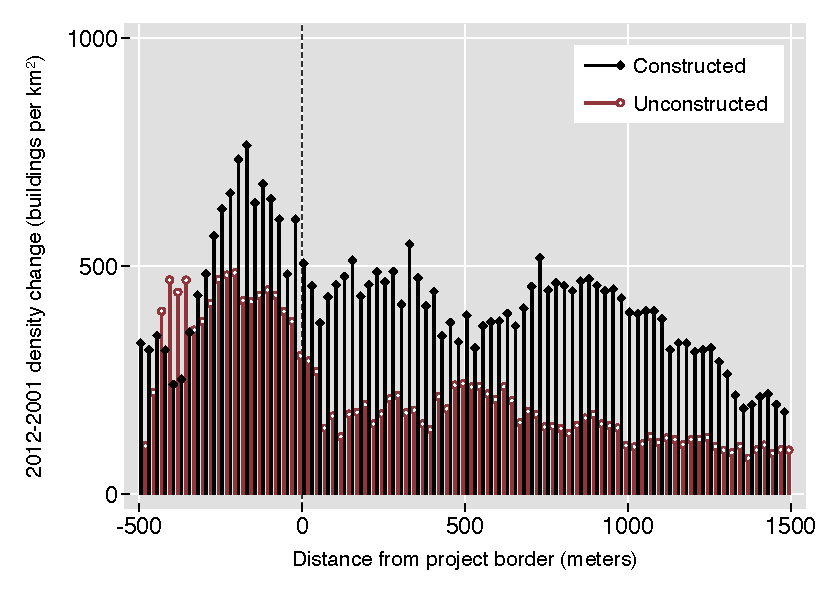
\includegraphics[width=\textwidth,trim={0.3cm .3cm 0.1cm 0cm}, clip=true]{figures/bblu_inf_rawchanges_4_2_spk.pdf}

%         \end{subfigure}
%         \begin{subfigure}[b]{0.48\textwidth}
%                     \caption[Network2]%
%             {{\footnotesize \textbf{Other} changes formal raw data}}   
%             \label{fig:prefor}
%             \centering
%             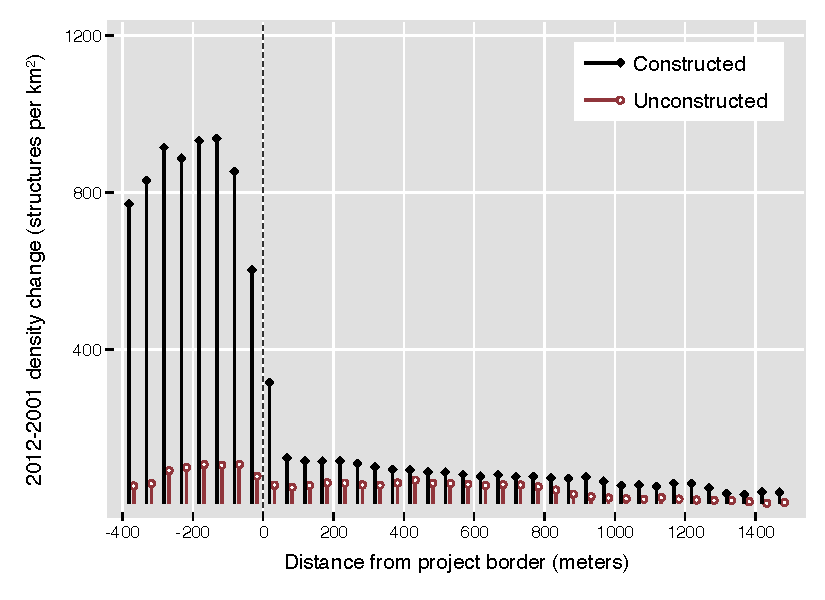
\includegraphics[width=\textwidth,trim={0.3cm .3cm 0.1cm 0cm}, clip=true]{figures/bblu_for_rawchanges_4_3_spk.pdf}

%         \end{subfigure}
%         \hfill
%         \begin{subfigure}[b]{0.48\textwidth} 
%                     \caption[]%
%             {{\footnotesize \textbf{Other} changes informal  raw data}}      
%             \label{fig:preinf} 
%             \centering 
%             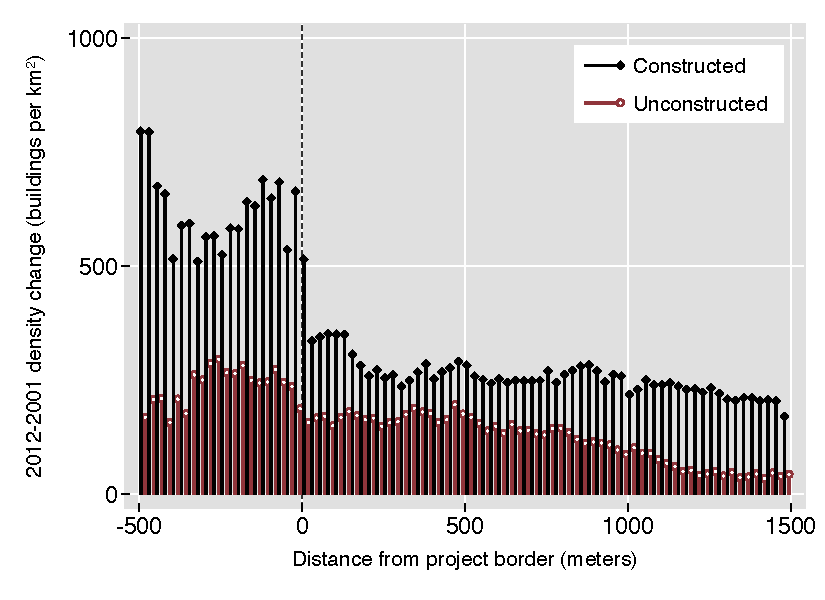
\includegraphics[width=\textwidth,trim={0.3cm .3cm 0.1cm 0cm}, clip=true]{figures/bblu_inf_rawchanges_4_3_spk.pdf}

%         \end{subfigure}
% \end{figure*}







\begin{table}
\caption{Building Density}
\begin{tabular}{lDDDDD}
\toprule
 & \small (1) & \small (2)  & \small (3) & \small (4) & \small (5) \\
 & Total & Formal  & Informal & Informal Bkyd. & Informal Non-Bkyd. \\ \midrule
\textbf{All Projects} \\inside project      &     798.586\textsuperscript{a}&     620.634\textsuperscript{a}&     177.952\textsuperscript{c}&     568.624\textsuperscript{a}&    -390.672\textsuperscript{a}\\
                    &   (147.475)                   &    (75.025)                   &   (102.386)                   &   (107.113)                   &    (82.015)                   \\[0.5em]
0-500m outside project &      48.071                   &      42.254\textsuperscript{c}&       5.817                   &      39.088                   &     -33.271                   \\
                    &    (60.616)                   &    (24.400)                   &    (50.920)                   &    (47.265)                   &    (27.170)                   \\[0.5em]
R$^2$               &       0.422                   &       0.394                   &       0.378                   &       0.328                   &       0.325                   \\

\midrule
\textbf{Greenfield} \\   inside project      &     566.673\textsuperscript{a}&     417.324\textsuperscript{a}&     149.349\textsuperscript{c}&     233.972\textsuperscript{b}&     -84.623                   \\
                    &   (200.320)                   &   (137.440)                   &    (86.149)                   &   (106.104)                   &    (59.202)                   \\[0.01em]
0-500m outside project &      44.501                   &      32.366                   &      12.135                   &      11.085                   &       1.050                   \\
                    &    (63.894)                   &    (31.149)                   &    (44.054)                   &    (41.479)                   &    (31.269)                   \\[0.8em] 
\textbf{In-Situ Upgrading} \\   inside project      &     768.386\textsuperscript{b}&     834.832\textsuperscript{a}&     -66.446                   &     763.886\textsuperscript{a}&    -830.332\textsuperscript{a}\\
                    &   (373.612)                   &   (149.444)                   &   (306.515)                   &   (275.248)                   &   (227.074)                   \\[0.01em]
0-500m outside project &     128.366                   &      91.173                   &      37.193                   &      79.348                   &     -42.155                   \\
                    &   (174.433)                   &    (83.033)                   &   (162.119)                   &   (145.311)                   &   (111.145)                   \\[0.8em]
\textbf{Other} \\   inside project      &     963.954\textsuperscript{a}&     692.627\textsuperscript{a}&     271.327\textsuperscript{c}&     707.612\textsuperscript{a}&    -436.284\textsuperscript{a}\\
                    &   (177.734)                   &    (77.008)                   &   (144.106)                   &   (124.715)                   &   (101.426)                   \\[0.01em]
0-500m outside project &      15.198                   &      34.208                   &     -19.010                   &      27.766                   &     -46.776                   \\
                    &    (85.359)                   &    (32.943)                   &    (72.308)                   &    (65.813)                   &    (33.342)                   \\[0.8em]
Mean Outcome 2001   &      526.22                   &      261.56                   &      264.66                   &       96.43                   &      168.23                   \\
Mean Outcome 2011   &      838.62                   &      385.14                   &      453.48                   &      286.79                   &      166.69                   \\
R$^2$               &       0.425                   &       0.396                   &       0.381                   &       0.336                   &       0.327                   \\
N                   &   1,705,534                   &   1,705,534                   &   1,705,534                   &   1,705,534                   &   1,705,534                   \\

\bottomrule
\end{tabular}
\end{table}





\begin{table}[h!] 
\caption{Effect of Housing Projects on Socio-demographics}
\label{table:sorting}
\small
\centering
%\caption{Census Composition Estimates }
\vspace{-2mm}
\begin{tabular}{lDDDDD}
\toprule
& \small (1) & \small (2) & \small (3) & \small (4)& \small (5)\\
& \small Age & \small P.O.B. not Gauteng & \small Unemployed & \small Years of Education & \small Monthly Income \\ \midrule 
\textbf{All Projects} \\inside project      &      -0.127                   &      -0.009                   &       0.017                   &       0.210                   &    1229.706\textsuperscript{b}\\
                    &     (0.288)                   &     (0.017)                   &     (0.020)                   &     (0.128)                   &   (563.606)                   \\[0.5em]
0-500m outside project &       0.026                   &       0.002                   &       0.004                   &      -0.007                   &     268.440                   \\
                    &     (0.267)                   &     (0.015)                   &     (0.018)                   &     (0.095)                   &   (606.673)                   \\[0.5em]
R$^2$               &       0.628                   &       0.742                   &       0.480                   &       0.659                   &       0.604                   \\

\midrule
\textbf{Greenfield} \\   inside project      &      -0.959                   &      -0.011                   &       0.064                   &      -0.082                   &     919.369                   \\
                    &     (0.679)                   &     (0.047)                   &     (0.042)                   &     (0.269)                   &   (802.935)                   \\[0.01em]
0-500m outside project &      -0.481                   &       0.018                   &       0.036                   &       0.156                   &     183.621                   \\
                    &     (0.519)                   &     (0.038)                   &     (0.038)                   &     (0.198)                   &   (699.540)                   \\[0.8em] 
\textbf{In-Situ Upgrading} \\   inside project      &       0.374                   &       0.015                   &      -0.008                   &       0.161                   &     405.889                   \\
                    &     (0.459)                   &     (0.021)                   &     (0.033)                   &     (0.202)                   &   (851.401)                   \\[0.01em]
0-500m outside project &      -0.344                   &       0.010                   &      -0.005                   &      -0.084                   &    -371.770                   \\
                    &     (0.502)                   &     (0.021)                   &     (0.033)                   &     (0.167)                   &   (956.350)                   \\[0.8em]
\textbf{Other} \\   inside project      &      -0.097                   &      -0.021                   &       0.020                   &       0.250                   &    1868.993\textsuperscript{b}\\
                    &     (0.406)                   &     (0.024)                   &     (0.027)                   &     (0.185)                   &   (728.876)                   \\[0.01em]
0-500m outside project &       0.425                   &      -0.004                   &      -0.008                   &      -0.036                   &     747.243                   \\
                    &     (0.343)                   &     (0.019)                   &     (0.023)                   &     (0.130)                   &   (805.159)                   \\[0.8em]
Mean Outcome 2001   &       27.30                   &        0.37                   &        0.47                   &        8.27                   &    2,477.01                   \\
Mean Outcome 2011   &       28.30                   &        0.43                   &        0.33                   &        9.68                   &    4,486.48                   \\
R$^2$               &       0.631                   &       0.744                   &       0.482                   &       0.660                   &       0.608                   \\
N                   &      12,734                   &      12,727                   &      12,724                   &      12,728                   &      12,724                   \\

\bottomrule
\multicolumn{6}{l}{\footnotesize Standard errors clustered at the project level in parenthesis. \textsuperscript{c} p$<$0.10, \textsuperscript{b} p$<$0.05, \textsuperscript{a} p$<$0.01  }\\
\multicolumn{6}{l}{\footnotesize P.O.B. means ``place of birth.''  Monthly income is in Rands.}
\end{tabular}
\end{table}








\begin{landscape}
{\footnotesize

\begin{table}[]
\small
\centering
\caption{Census Household-level Estimates }\label{table:censusestimates}
\vspace{-2mm}
\resizebox{.9\linewidth}{!}{
\begin{tabular}{lDDDDDDDD}
\toprule
 & \small (1) & \small (2)  & \small (3) & \small (4) & \small (5)  & \small (6)  & \small (7) & (8)\\
 & \small Flush Toilet & \small Water Indoors  & \small Electricity Cooking & \small Electricity Heating & \small Electricity Lighting  & \small Number of Rooms  & \small Household Size & Population Density\\ \midrule 
\textbf{All Projects} \\inside project      &       0.109                   &       0.123\textsuperscript{a}&       0.167\textsuperscript{b}&       0.102                   &       0.058                   &       0.153                   &       0.104                   &    -879.717                   \\
                    &     (0.077)                   &     (0.043)                   &     (0.076)                   &     (0.070)                   &     (0.077)                   &     (0.156)                   &     (0.098)                   &  (1258.435)                   \\[0.5em]
0-500m outside project &      -0.004                   &       0.020                   &       0.031                   &       0.020                   &       0.009                   &       0.103                   &       0.029                   &    -888.850                   \\
                    &     (0.033)                   &     (0.037)                   &     (0.041)                   &     (0.045)                   &     (0.031)                   &     (0.111)                   &     (0.057)                   &   (818.819)                   \\[0.5em]
R$^2$               &       0.529                   &       0.541                   &       0.582                   &       0.548                   &       0.555                   &       0.631                   &       0.632                   &       0.561                   \\

\midrule
\textbf{Greenfield} \\   inside project      &       0.122                   &       0.113                   &       0.171                   &       0.099                   &       0.153                   &       0.380                   &       0.167                   &    3328.827                   \\
                    &     (0.107)                   &     (0.111)                   &     (0.112)                   &     (0.130)                   &     (0.096)                   &     (0.286)                   &     (0.166)                   &  (2525.594)                   \\[0.01em]
0-500m outside project &      -0.035                   &       0.020                   &      -0.018                   &       0.006                   &       0.029                   &       0.181                   &       0.138                   &   -3251.609                   \\
                    &     (0.047)                   &     (0.063)                   &     (0.063)                   &     (0.074)                   &     (0.054)                   &     (0.250)                   &     (0.142)                   &  (2315.189)                   \\[0.8em] 
\textbf{In-Situ Upgrading} \\   inside project      &       0.303\textsuperscript{b}&       0.119                   &       0.134                   &       0.106                   &       0.043                   &       0.125                   &       0.096                   &   -4073.231                   \\
                    &     (0.153)                   &     (0.088)                   &     (0.130)                   &     (0.117)                   &     (0.105)                   &     (0.236)                   &     (0.185)                   &  (2913.004)                   \\[0.01em]
0-500m outside project &       0.000                   &      -0.024                   &       0.024                   &       0.003                   &      -0.005                   &      -0.290                   &      -0.045                   &    -397.793                   \\
                    &     (0.077)                   &     (0.085)                   &     (0.095)                   &     (0.108)                   &     (0.065)                   &     (0.242)                   &     (0.106)                   &  (1800.869)                   \\[0.8em]
\textbf{Other} \\   inside project      &      -0.028                   &       0.148\textsuperscript{a}&       0.159                   &       0.089                   &       0.034                   &       0.065                   &       0.060                   &    -209.749                   \\
                    &     (0.103)                   &     (0.052)                   &     (0.114)                   &     (0.104)                   &     (0.122)                   &     (0.230)                   &     (0.128)                   &  (1032.197)                   \\[0.01em]
0-500m outside project &      -0.005                   &       0.053                   &       0.035                   &       0.023                   &       0.002                   &       0.288\textsuperscript{b}&       0.008                   &    -986.542                   \\
                    &     (0.046)                   &     (0.045)                   &     (0.045)                   &     (0.049)                   &     (0.038)                   &     (0.144)                   &     (0.068)                   &   (829.532)                   \\[0.8em]
Mean Outcome 2001   &        0.79                   &        0.35                   &        0.66                   &        0.62                   &        0.77                   &        3.30                   &        3.51                   &    8,566.83                   \\
Mean Outcome 2011   &        0.83                   &        0.54                   &        0.81                   &        0.72                   &        0.82                   &        3.56                   &        3.18                   &    9,823.82                   \\
R$^2$               &       0.541                   &       0.551                   &       0.589                   &       0.555                   &       0.562                   &       0.634                   &       0.634                   &       0.563                   \\
N                   &      12,732                   &      12,732                   &      12,732                   &      12,732                   &      12,732                   &      12,709                   &      12,730                   &      12,734                   \\

\bottomrule
\multicolumn{9}{l}{\footnotesize All regressions include 3km grid Fixed-Effects. Standard errors clustered at the project level in parenthesis. \textsuperscript{c} p$<$0.10,\textsuperscript{b} p$<$0.05,\textsuperscript{a} p$<$0.01 }
\end{tabular}
}
\end{table}

}
\end{landscape}




\begin{table}
\small
\centering
\caption{Triple Difference Estimates on Log-Prices}\label{table:priceDDD_het}
\vspace{-2mm}
\begin{tabular}{lCC}
\toprule
 & \small (1) & \small (2)  \\ \midrule 
 \textbf{All Projects} \\
 inside project      &      -0.192                   &      -0.169                   \\
                    &     (0.231)                   &     (0.228)                   \\[0.5em]
0-500m outside project &      -0.074                   &      -0.072                   \\
                    &     (0.058)                   &     (0.058)                   \\[0.5em]
Lot Size Controls   &                               &  \checkmark                   \\
r2                  &        0.45                   &        0.45                   \\
N                   &      67,751                   &      67,751                   \\

 \midrule
\textbf{Greenfield} \\   inside project      &       0.172                   &       0.113                   \\
                    &     (0.168)                   &     (0.152)                   \\[0.01em]
0-500m outside project &       0.034                   &       0.035                   \\
                    &     (0.112)                   &     (0.112)                   \\[0.8em]
\textbf{In-Situ Upgrading} \\   inside project      &       0.424\textsuperscript{b}&       0.495\textsuperscript{b}\\
                    &     (0.188)                   &     (0.197)                   \\[0.01em]
0-500m outside project &      -0.157                   &      -0.160                   \\
                    &     (0.110)                   &     (0.110)                   \\[0.8em]
\textbf{Other} \\   inside project      &      -0.412                   &      -0.373                   \\
                    &     (0.309)                   &     (0.302)                   \\[0.01em]
0-500m outside project &      -0.022                   &      -0.017                   \\
                    &     (0.082)                   &     (0.082)                   \\[0.8em]
Lot Size Controls   &                               &  \checkmark                   \\
r2                  &        0.45                   &        0.46                   \\
N                   &      67,751                   &      67,751                   \\

\bottomrule
\multicolumn{3}{l}{\footnotesize Standard errors clustered at the project level in parenthesis.} \\
\multicolumn{3}{l}{ \textsuperscript{c} p$<$0.10,\textsuperscript{b} p$<$0.05,\textsuperscript{a} p$<$0.01 }
\end{tabular}
\end{table} 

% \begin{figure}
% 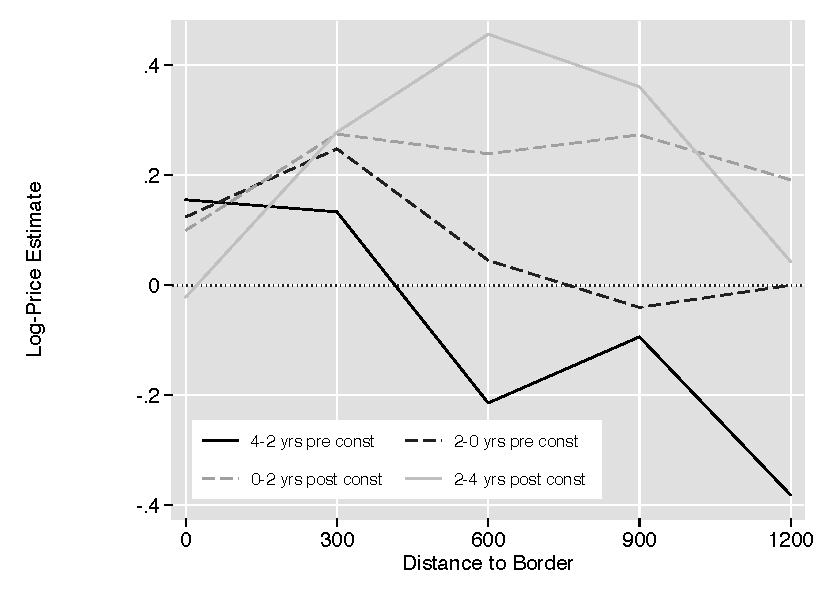
\includegraphics{figures/price_to_event_30.pdf}
% \end{figure}


\end{document}


